\documentclass[10pt,a4paper]{article}
\usepackage[utf8]{inputenc}
\usepackage[spanish]{babel}
\usepackage{amsmath}
\usepackage{amsfonts}
\usepackage{amssymb}
\usepackage{graphicx}
\usepackage[left=2cm,right=2cm,top=2cm,bottom=2cm]{geometry}


\begin{document}

\begin{titlepage}
\title{\textbf{
	{\Huge Encapsular el acceso a una aplicación BASIC/MS-DOS}\\
	{\Large Sistemas Legados}
}}
\author{
	Pedro Allué Tamargo (758267)
	\and
	Juan José Tambo Tambo (755742)
	\and
	Jesús Villacampa Sagaste (755739)
}
\date{\today}
\clearpage\maketitle
\thispagestyle{empty}
\tableofcontents
\end{titlepage}


\section{Introducción}

En esta práctica se pide la realización de un \emph{wrapper} sobre una aplicación legada de un sistema \emph{MS-DOS}. Para ello se va a utilizar un emulador y mediante capturas de pantallas de la interacción con la misma y un software de reconocimiento de caracteres (\emph{OCR}) se van a extraer los datos.


\section{Esfuerzos invertidos}

\begin{itemize}
\item Pedro Allué Tamargo:
\item Juan José Tambo Tambo:
\item Jesús Villacampa Sagaste:
\end{itemize}

\section{Descripción de la aplicación legada}

Para interaccionar con la aplicación legada se va a utilizar el emulador \emph{DosBox} (el incluido junto al enunciado de la práctica). Para ejecutar la aplicación se va a ejecutar el \emph{script} \texttt{database.bat} que ejecuta el emulador y la aplicación legada.\\
La aplicación legada consiste en un programa de \emph{MS-DOS} que gestiona una biblioteca de cintas con distintos programas y/o juegos (Figura \ref{fig:aplicacion_legada}).

\begin{figure}[h!]
\centering
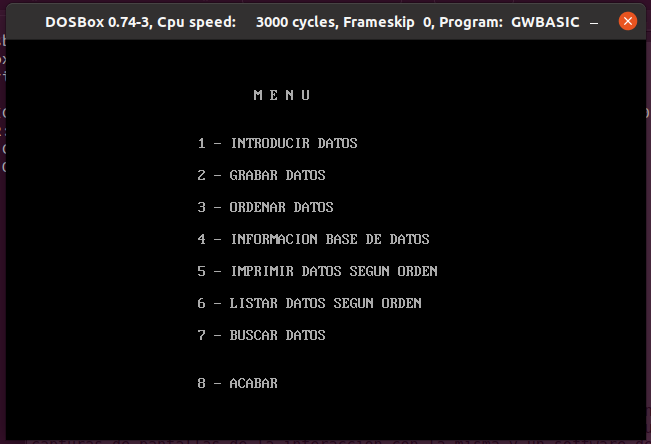
\includegraphics[scale=0.5]{images/aplicacion_legada.png}
\caption{Captura de pantalla del menú principal de la aplicación legada}
\label{fig:aplicacion_legada}
\end{figure}

Con esta aplicación el usuario podía introducir nuevos registros que hacían alusión a cintas con los campos: \emph{Nombre}, \emph{Tipo}, \emph{Cinta}. También se añade un campo que gestiona la propia aplicación correspondiente al número de registro que le corresponde en la base de datos.


\section{Tecnología elegida}


\section{Implementación del Wrapper}
\subsection{Preparación del entorno}

Ficheros de configuración aquí.


\subsection{Frontend del Wrapper}


\subsection{Backend del Wrapper}




\end{document}